\documentclass[12pt]{amsart}

%Below are some necessary packages for your course.
\usepackage{amsfonts,latexsym,amsthm,amssymb,amsmath,amscd,euscript,tikz}
\usepackage{framed}
\usepackage{fullpage}
\usepackage{comment}
\usepackage{tikz}
\usepackage{bm}
\usepackage{enumerate}
\usepackage{dsfont}
\usepackage{hyperref}
\usetikzlibrary{patterns}
\usepackage{subfig}
\usepackage{float}
\usepackage{listings}
% \usepackage[cache=false]{minted}

\lstset{
  basicstyle=\footnotesize,
  xleftmargin=.2\textwidth, xrightmargin=.2\textwidth
}

\usetikzlibrary{decorations.markings,decorations.pathmorphing}
\usepackage{tikz-cd}
\usepackage{enumitem}
\usepackage{hyperref}
    \hypersetup{colorlinks=true,citecolor=blue,urlcolor =blue,linkbordercolor={1 0 0}}

\newenvironment{statement}[1]{\smallskip\noindent\color[rgb]{0.0,0.0,0.0} {\bf #1.}}{}
\allowdisplaybreaks[1]

%Below are the theorem, definition, example, lemma, etc. body types.

\newtheorem{theorem}{Theorem}
\newtheorem*{proposition}{Proposition}
\newtheorem{lemma}[theorem]{Lemma}
\newtheorem{corollary}[theorem]{Corollary}
\newtheorem{conjecture}[theorem]{Conjecture}
\newtheorem{postulate}[theorem]{Postulate}
\theoremstyle{definition}
\newtheorem{defn}[theorem]{Definition}
\newtheorem{example}[theorem]{Example}

\theoremstyle{remark}
\newtheorem*{remark}{Remark}
\newtheorem*{notation}{Notation}
\newtheorem*{note}{Note}

% You can define new commands to make your life easier.
\newcommand{\BR}{\mathbb R}
\newcommand{\BC}{\mathbb C}
\newcommand{\BF}{\mathbb F}
\newcommand{\BQ}{\mathbb Q}
\newcommand{\BZ}{\mathbb Z}
\newcommand{\BN}{\mathbb N}
\newcommand{\BE}{\mathbb E}

\newcommand{\CU}{\mathcal{U}}
\newcommand{\CO}{\mathcal{O}}
\newcommand{\CC}{\mathcal{C}}
\newcommand{\Ob}{\operatorname{Ob}}
\newcommand{\Mor}{\operatorname{Mor}}


% We can even define a new command for \newcommand!
\newcommand{\C}{\mathbb{C}}
\newcommand{\F}{\mathbb{F}}
\newcommand{\Q}{\mathbb{Q}}
\newcommand{\Z}{\mathbb{Z}}
\newcommand{\R}{\mathbb{R}}
\newcommand{\N}{\mathbb{N}}
\newcommand{\bP}{\mathbb{P}}

\newcommand{\Hom}{\operatorname{Hom}}
\newcommand{\End}{\operatorname{End}}
\newcommand{\ch}{\operatorname{char}}
\newcommand{\image}{\operatorname{im}}
\newcommand{\kernel}{\operatorname{ker}}
\newcommand{\rank}{\operatorname{rank}}
\newcommand{\sym}{\operatorname{Sym}}
\newcommand{\im}{\operatorname{im}}
\newcommand{\lcm}{\operatorname{lcm}}
\newcommand{\Res}{\operatorname{Res}}

\newcommand{\Pois}{\text{Pois}}
\newcommand{\ex}{\text{exp}}
\newcommand{\Var}{\text{Var}}
\newcommand{\Binom}{\text{Binom}}
\newcommand{\btheta}{\bm\theta}
\newcommand{\bT}{\bm T}
\newcommand{\E}{\mathbb{E}}
\newcommand{\I}{\mathbb{I}}
\newcommand{\BP}{\mathbb{P}}
\newcommand{\x}{\bm x}
\newcommand{\y}{\bm y}
\newcommand{\z}{\bm z}
\newcommand{\bmT}{\bm T}
\newcommand{\bmX}{\bm X}
\newcommand{\bmY}{\bm Y}
\newcommand{\bmZ}{\bm Z}
\newcommand{\br}{\bm r}
\newcommand{\bI}{\bm I}
\newcommand{\1}{\mathds{1}}



% If you want a new function, use operatorname to define that function (don't use \text)

\renewcommand{\baselinestretch}{1.25}

\title{CS 182 Fall 2022, Problem Set 1}

\begin{document}

\maketitle

\vspace*{-0.25in}
\centerline{Due: September 27, 2022 11:59pm}

\begin{center}
\end{center}
\vspace*{0.15in}

\noindent This problem set covers Lectures 2, 3, and 4. The topics include Uninformed Search, Informed Search, and Motion Planning.
\vspace*{0.35in}

\begin{statement}{1}
\textit{Uninformed and Informed Search.} (7 points)

\begin{enumerate}
    \item  For each of the following, explain why it's true or provide a counterexample.
    \begin{enumerate}
        \item (1 point) Breadth-first search is a special case of uniform-cost search.
        \\If uniform-cost search is applied on a problem where the action-costs from state to state are all the same, then the path-cost function (that 
        dictates how nodes are expanded) simply returns the depth at which the node is found at. Hence, nodes are expanded based on the order in which they 
        were first encountered, which is exactly a Breadth-first search.
        \item (1 point) Uniform-cost search is a special case of A* search. %3.22
        \\ If we let $h(n) = 0$ in the evaluation function $f(n) = g(n) + h(n)$ then $f(n) = g(n)$. $g(n)$ is the path-cost from the inital state to 
        $n$, so nodes are expanded based on path-cost alone. which is how Uniform-cost search expands nodes.
        \item (1 point) Depth-first search always expands at least as many nodes as A* search with an admissible heuristic.
        \\Consider the following search space with initial state $S$ and goal state $G$: 
        \begin{center}
            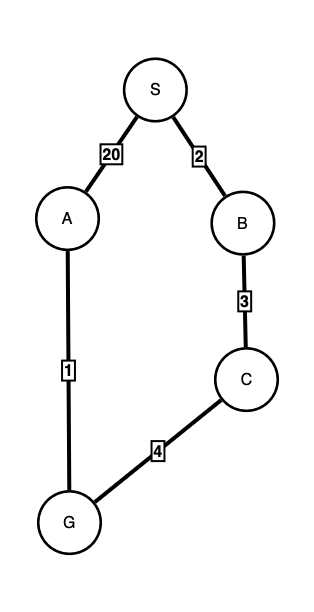
\includegraphics[width=0.3\textwidth]{images/graph.png}
        \end{center}
        Also, define $h(A) = 1, h(B) = 8, h(C)=6,$ and $h(G)= 0$. A depth-first search that expands left-most modes first only expands $S$ and $A$ 
        before encountering $G$ and returning. A* search, on the other hand, expands $S$, $B$, and $C$ before expanding $G$ and returning. Hence, depth-first search does not 
        always expand at least as many nodes as A*.
        \item (1 point) Breadth-first search is complete even if zero step costs are allowed. 
        \\ This is true because Breadth-first search only considers the depth in the tree at which nodes were encountered when choosing what node to 
        expand next, so every node at every level of the tree is still expanded, making this a complete search. 
        \item (1 point) Assume that a rook can move on a chessboard any number of squares in a straight line, vertically or horizontally, but cannot jump over other pieces. Manhattan distance is an admissible heuristic for the problem of moving the rook from square A to square B in the smallest number of moves.
        \\ Suppose a rook wanted to move from square $A$ to square $B$ and that square $A$ and square $B$ are are on opposite sides of the same column, with no pieces in between. Then, the least number of 
        moves to get the rook from $A$ to $B$ is 1 because the rook can move any number of moves in a straight line, which $A$ and $B$ are on, but the manhattan distance between these two squares is the width of the board - 1. This heuristic overestimates 
        the cost, so it is not admissible. 
    \end{enumerate}
    \item (2 points) Describe a state space in which iterative deepening search performs much worse than depth-first search (for example, $\Theta(n^2)$ vs. $\Theta(n)$).
    \\ First, we assume that DFS and IDS expand left-most nodes first. Now, suppose we have a finite state space where each state has $b$ successors and the 
    goal is at level $d$. Specifically, the solution is the left-most node on level $d$. In this state space, DFS finds the goal after just $d $ actions, which is 
    $O(d)$ time. IDS, on the other hand, has to try all the depth levels from $1$ to $d-1$ before finally reaching depth level $d$ and finding the goal. So IDS expands the $b$ children of the root $d$ times, the $b^2$ nodes on the next level $d-1$ times, and so on and so forth. 
    So the number of nodes expanded is 
    \begin{align*}
        bd + b^2(d - 1) + b^3 (d - 2) + ... + 2b^{d - 1}
    \end{align*}
    , which is $O(b^d)$ asymptotically. This is much worse than $O(d)$. 

\end{enumerate}


\end{statement}


\newpage
\begin{statement}{2} 
\emph{Gridworld.} (13 points) Consider the unbounded version of the regular 2D grid. The start state is at the origin, $(0,0)$, and the goal state is at $(u, v)$. You may assume every edge is bidirectional and has unit cost. You should provide justifications for your answers. Below is an example image showing what this arrangement would look like if $(u, v) = (8,5)$. Be sure the consider the generic coordinates $(u, v)$ for the questions below.
\begin{figure}[H]
    \centering
    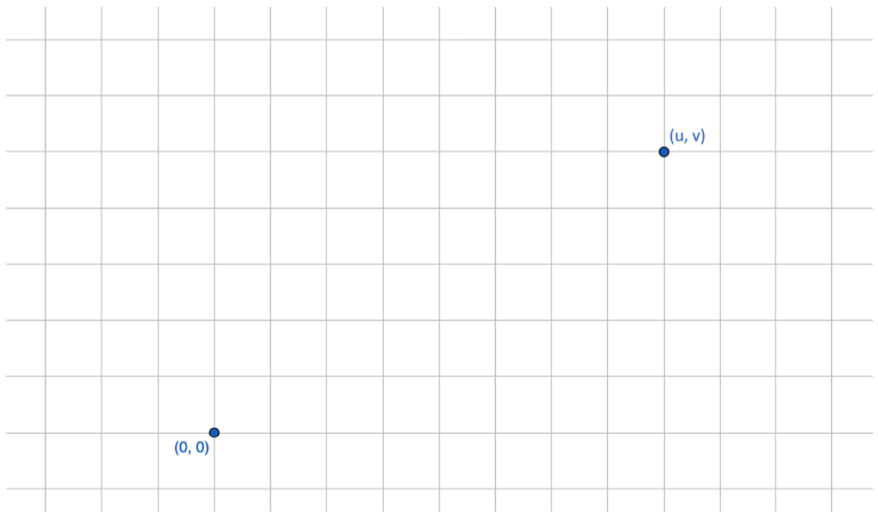
\includegraphics[width=0.8\textwidth]{images/2d_grid_new.png}
\end{figure}

\begin{enumerate}
    \item (1 point) What is the branching factor $b$ in this state space? In other words, for each state, how many neighbors does that state have? 
    \\ $b = 4$ 
    \item (2 points) Is $h(x,y) = |x - u| + |y - v|$ an admissible heuristic for a state at $(x, y)$? Is it a consistent heuristic?
    \\ The heuristic is admissible. The fornula for the heuristic is the Manhattan Distance from $(x, y)$ to $(u, v)$, which, on a 2D grid, is the shortest 
    distance from any two points when you can only move at right angles along the axes. Because each move costs one unit, the cost of the optimal path from a state to the goal is 
    equal to the manhattan distance. The heuristic is also consistent: in this search space, 2 of the 4 possible moves on state $(x, y)$ inch us closer toward the goal by one unit and 
    2 of the moves put us farther away by one unit. First, assume action $a$ moves us in a direction opposite the goal from state $(x, y)$ to $(x', y')$.
    Then, 
    \begin{align*}
        c((x, y), a, (x', y')) + h((x', y')) &= 1 + (h((x, y)) + 1)\\ &> h((x, y))
    \end{align*}
    Now, suppose that action $a$ moves us closer to the goal. Then, 
    \begin{align*}
        c((x, y), a, (x', y')) + h((x', y')) &= 1 + (h((x, y)) - 1)\\ &= h((x, y))
    \end{align*}
    Hence, $h$ is consistent.
    \item (2 points) What is the maximum number of nodes expanded by A* Graph Search using $h$?\footnote{\label{max}``maximum" refers to worst-case tie-breaking, i.e. when choosing among states with the same desirability as the goal state, assume the goal state is chosen last.}
    \\ First, assume that the goal state is not on the $x$ or $y$ axes: A* search trivially finds the optimal path in the least number of steps. 
    When the goal state, $(u, v)$, is not on the $x$ or $y$ axes, there are two moves from the initial state that move us further from the goal and two moves that move us toward the goal. 
    Suppose $(x, y)$ is a successor of the initial state and is caused by a move that moves us further from the goal state. Then, 
    \begin{align*}
        f((x, y)) &= g((x, y)) + h((x, y)) \\ 
        &= 1 + (h((x, y)) + 1)\\ 
        &= h((x, y)) + 2
    \end{align*}
    Now, suppose $(x, y)$ is a successor of the initial state and is caused by a move that moves us toward from the goal state. Then,
    \begin{align*}
        f((x, y)) &= g((x, y)) + h((x, y)) \\ 
        &= 1 + (h((x, y)) - 1)\\ 
        &= h((x, y))
    \end{align*}
    Then A* only ever expands nodes that move us toward the initial state, of which there are $u*v$ possible nodes. In fact, for any node $(x, y)$ in that set, we have that 
    \begin{align*}
        f((x, y)) &= g((x, y)) + h((x, y))\\ 
        &= (|x - 0| + |y - 0|) + (|u - x| + |v - y|) \\ 
        &= u + v
    \end{align*}
    Where $g((x, y)) = |x - 0| + |y - 0|$ because the only way to get from the initial state to $(x, y)$ is by moving at right angles along the axes. This proves that all $u*v$ nodes have 
    the same $f(n)$ value so in the worst case scenario, A* expands all $u*v$ nodes!
    \item (1 point) Does $h$ remain admissible if some links are removed?
    \\ Yes because if links are removed then we would have to perform extra moves and expand more nodes than the heuristic suggests, so the heuristic is still an underestimate and therefore still 
    admissible. 
    \item (1 point) Does $h$ remain admissible if some links are added between nonadjacent states? % add consistency
    \\ No. For example, if a link was added from a neighbor of the initial state to the goal state and if we gave this link unit cost, then 
    the heuristic would overestimate the path-cost for that node. 
    \item (6 points) Take $h_2(x,y) = \sqrt{h(x,y)}$ with the original search space. Is $h_2$ admissible? Is it consistent?\\ 
    \\ Let $C*_{x, y}$ be the optimal cost from state $(x, y)$ to the goal. From part 1, we know that the optimal cost from 
    state $(x, y)$ to the goal IS the manhattan distance, $h((x, y))$, so $C*_{x, y} = h((x, y))$. Then, for all $(x, y)$ we have 
    \begin{align*}
        h_2((x, y)) &= \sqrt{h((x, y))} \\ 
        &\leq h((x, y))\\ 
        & \leq C*_{x, y}
    \end{align*}
    so the heuristic is admissible. \\ 
    Also from above, we know that an action either moves us either away from or toward the goal. Consider the former: given state 
    $(x, y)$ we consider an action, $a$, that moves us to a state $(x', y')$ away from the goal. Then, 
    \begin{align*}
        c((x, y), a, (x', y')) + h_2((x', y')) &= 1 + \sqrt{h((x', y'))} \\ 
        &= 1 + \sqrt{(1 + h((x, y)))} \\ 
        &> \sqrt{h((x, y))} \\ 
        = h_2((x, y))\\ 
    \end{align*}
    Now, we consider the latter: given state 
    $(x, y)$ we consider an action, $a$, that moves us to a state $(x', y')$ toward the goal. \\Then, 
    \begin{align*}
        c((x, y), a, (x', y')) + h_2((x', y')) &= 1 + \sqrt{h((x', y'))} \\ 
        &= 1 + \sqrt{h((x, y)) - 1} \\ 
        &\geq \sqrt{h((x, y))} \\ 
        &= h_2((x, y)) 
    \end{align*}
    So, $\forall (x, y)$ and action $a$, it holds that $c((x, y), a, (x', y')) + h_2((x', y')) \geq h(x, y)$, therefore, the heuristic is 
    consistent.
\end{enumerate}
\end{statement}

\newpage
\begin{statement}{3} \textit{Informed Search.} (20 points) Let $h^*(x)$ denote the cost function that returns the shortest distance between a state $x$ and the nearest goal state $t$. Let $h(\cdot)$ be a heuristic that overestimates $h^*(\cdot)$ by at most $\epsilon$, meaning that for all states $x$, $h(x) \leq h^*(x) + \epsilon$. Assume that $h(\cdot)$ assigns $0$ to any goal state. Prove that A$^*$ \textit{tree search} using $h$ finds a path to the nearest goal state $t$ whose cost is at most $\epsilon$ more than an optimal path to the nearest goal state. Formally, if $s$ is the start state, $t$ is the goal state returned by $A^*$ search, and $g(x)$ denotes the lowest cost path from $s$ to $x$ along the explored graph, then show that $g(t) \leq h^*(s) + \epsilon$.

\end{statement}

\newpage
\begin{statement}{4}
\emph{Motion Planning.} (20 points)
Let $S$ be a set of disjoint obstacles (simple polygons) in the plane, and let $n$ denote the total number of their
edges. Assume that we have a point robot moving on the plane that can touch the edges of the obstacles.
(That is, we treat the obstacles as open sets.) The robot starts at the $p_{start}$ position and must get to the
$p_{goal}$ position using the shortest collision-free path. In class, we proved that any shortest path between $p_{start}$
and $p_{goal}$ is a polygonal path whose inner vertices are the vertices of the obstacles. You may use this result
in your answer to the following questions.

\begin{figure}
    \centering
    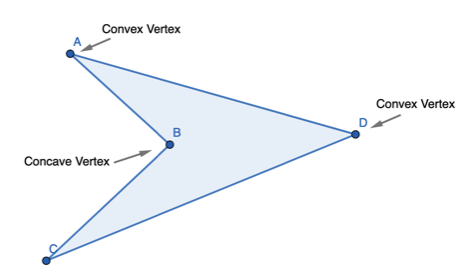
\includegraphics[width=0.5\textwidth]{images/convex-concave.png}
    \caption{Examples of Convex and Concave Vertices}
    \label{fig:convex-concave}
\end{figure}

We now consider two different kinds of vertices on obstacles.
\begin{itemize}
    \item  A vertex whose internal angle formed by its two edges is less than $180^\circ$ is called \textit{convex}.
    \item A vertex whose internal angle formed by its two edges is at least $180^\circ$ is called \textit{concave}.
\end{itemize}
See Fig. \ref{fig:convex-concave}.\\

\noindent
Prove that a shortest path from $p_{start}$ to $p_{goal}$ is a polygonal path where each inner vertex (if any) corresponds to a \emph{convex} vertex of some obstacle.  \\
\noindent\textbf{Hint:} Think about what will happen if there is a shortest path from $p_{start}$ to $p_{goal}$ where one inner vertex is a polygon's concave vertex.
\end{statement}


\newpage
\begin{statement}{5}
\emph{Programming.} (35 points) Your friend has a hobby of collecting gnomes and giving them mini-houses within her garden. Moreover, she has a robot that she intends to use to visit each of the gnomes each week to present them with fresh flowers. Your friend wants you to help her program the robot to figure out a fast route to get to every gnome residence. The garden is a 2D rectangular grid divided into discrete squares. Each square is either free, a vegetable (i.e. an obstacle), or a gnome residence. The route must visit every gnome residence at least once. A goal node is any node
where the robot has already visited every residence at least once.
The size of the grid will vary depending on which part you are working on, but you are guaranteed that there are no more than 5 residences.
Your task is to tell the gnome which set of actions it should take to accomplish its goal.\\

\noindent
As a visual reference, here is an ASCII rendition of a neighborhood map with 2 residences (labeled $R$) and some
walls (labeled $O$):

\begin{lstlisting}
                S.O.O
                ..O.R
                O.O.O
                .R..R
\end{lstlisting}

\noindent
This will be represented in the code as a list of lists, with blank spaces being 0, obstacles being -1 and
residences being 1. The exact structure for the map above is

\begin{lstlisting}
                [[0,0,-1,0,-1],
                [0,0,-1,0,1],
                [-1,0,-1,0,-1],
                [0,1,0,0,1]]
\end{lstlisting}

\noindent
The start position is given as a tuple of row-column coordinates; the start position is $(0,0)$ for this grid.
The cost is uniformly $1$ for every attempted move. The robot can only move in the 4 cardinal directions
(up, right, down, left), and cannot move off of the grid. Trying to move into obstacles or off the grid results in staying put.\\

\noindent
A node should encompass the current position of the robot, as well as which residences have been visited and which have not. Two nodes with the same position, but different visited residences are different nodes.
Note, when adding successors of a search node onto your priority queue, make sure to add them in the
following order: up, right, down, left, so that they will be explored in that order. Tie-breaking for $A^*$ should be done by favoring nodes added earlier. Tie-breaking for BFS is the same; however tie-breaking for DFS, if using a stack, should result in adding the successors in the reverse order such that the successors will be visited in the correct order. \\


\noindent
For example inputs and outputs, see \verb|pset1_sample_test_case1.txt|. The first line contains the number of rows $r$ and columns $c$. The next $r$ lines contain the map information. The last line contains the coordinates for the start state $(r_0, c_0)$. You may also use any of the python standard libraries as you see fit.
\end{statement}

\begin{enumerate}
    \item (12 points, graded jointly with 5.2)
\textit{Defining the search problem.} 
The goal of this part of the problem is to describe our problem as just an instance of the graph search problem. How  do we do this (i.e. what are the nodes and edges of the graph that we can search to find a solution)? In addition to answering this in your writeup, fill in the methods of \texttt{GridworldSearchProblem}, which inherits from the abstract class \texttt{SearchProblem}.
    \item (4 points, graded jointly with 5.1) \emph{DFS}. For the remaining parts, your implementation of the search strategies should not depend on your implementation of\\ \texttt{GridWorldSearchProblem} and should instead work only by calling the methods of \texttt{SearchProblem} (i.e. treating the search problem as an abstract class). 
    Implement depth-first search in the function \texttt{depthFirstSearch(problem)}. Note that you should only do cycle detection and not re-expand any nodes along a single path; your algorithm should allow for the same node to be
    visited by different paths. Cycle detection preserves the low memory requirements of DFS.
    \item (4 points) \emph{BFS}. Implement breadth-first search in the \texttt{breadthFirstSearch(problem)} function. Note that you should globally keep track of visited nodes and not expand any node more than once.
    \item (6 points, graded jointly with 5.5)
\emph{A*}. Implement A* search in the\\ \texttt{aStarSearch(problem, heuristic)} function. The \texttt{heapq} module is one possible way to implement your priority queue. Alternatively, feel free to use the data structures we have provided. The \texttt{heuristic} parameter should be a function that returns a numeric value. The autograder will test your A* function with the \texttt{nullHeuristic} that always returns 0. Note that this trivial heuristic is consistent. For debugging, we recommend using the \texttt{nullHeuristic} since with this, the \texttt{aStarSearch} should do the same thing as the \texttt{breadthFirstSearch}.
    
    \item (3 points, graded jointly with 5.4) \emph{Simple Heuristic}. Now you will implement heuristics, which may depend on how you implemented your states. 
 Your simple heuristic should return the number of residences that haven't been visited. Implement this in the function \texttt{simpleHeuristic(state, problem)}. The autograder will test this by passing your heuristic as the \texttt{heuristic} parameter in your A* function.

    \item (6 points, 5 bonus points)
\emph{Custom Heuristic Challenge}. The simple heuristic is quick to compute, but not very effective in guiding A*. Try to come up with your own heuristic that reduces the number of nodes expanded. Your heuristic should be consistent. In your writeup, you should prove that your custom heuristic is consistent. Implement this in the \texttt{customHeuristic(state, problem)}
function. The autograder will test this by passing your \texttt{customHeuristic(state, problem)} as the \texttt{heuristic} parameter in your A* function. You will get full marks by expanding fewer nodes than the simple heuristic. Moreover, we will have a competition with a leaderboard on Gradescope to see who has the best heuristic!
Concretely, students will be ranked on the leaderboard to see who expands the least number of nodes over our hidden test cases.
We also have a column in the leaderboard for overall execution time as well.
Under ``leaderboard name", feel free to either use your name or a pseudonym.
The top 5 submissions on the leaderboard according to least number of nodes expanded will receive 5 bonus points on this problem set (as well as bragging rights for best heuristic)!
\end{enumerate}


\newpage
\begin{statement}{6}
\noindent \textbf{Collaboration, Calibration and References}. (5 points)
\begin{enumerate}
    \item With whom did you work on this problem set? What (if any) references and/or resources did you use beyond the course lecture slides and textbook? 
    \item (5 points) Approximately how long did it take you to complete this problem set? Please complete this brief \href{https://forms.gle/TbUE8je3Rb2oG4Us9}{survey} worth 5 points, graded for completion.
\end{enumerate}
\end{statement}


\end{document}



